\section{Funções de Engenharia}

Para cada função existente no projeto, as entradas, saídas e definições de retorno são descritas a seguir. Algumas rotinas recuperam informações do banco de dados local ou das bibliotecas utilizadas, enquanto outras calculam diretamente parâmetros de projeto.

A organização da engenharia segue a sequência de transporte de fluidos, bombas, propriedades termofísicas, reatores e balanço de massa. Essa ordem explicita a progressão dos fundamentos físicos até os modelos de cálculo utilizados pelo \textit{software}.

\subsection{Transporte de Fluidos}

\subsubsection{Dimensionamento de Tubulações}

Tubulações são componentes por onde o fluido escoa, permitindo a transferência de matéria entre equipamentos, desde a entrada de matéria-prima até a saída de produtos. Seu correto dimensionamento é imprescindível para a segurança e a eficiência do processo.

O dimensionamento consiste em definir o diâmetro nominal e o \textit{schedule} capazes de conduzir as vazões dentro de faixas de velocidade e perda de carga economicamente ótimas. As grandezas envolvidas incluem vazão (mássica ou volumétrica), velocidade admissível, propriedades do fluido (massa específica, viscosidade), comprimento equivalente (devido a acessórios) e características do material (rugosidade, pressão de projeto).

Na prática, calcula-se um diâmetro a partir da vazão e velocidade alvo e seleciona-se o diâmetro comercial imediatamente superior disponível, verificando em seguida a perda de carga pelo método de Darcy–Weisbach e a integridade mecânica conforme normas aplicáveis. Temperatura e pressão afetam propriedades físicas do fluido e critérios de espessura da tubulação; adicionalmente, a topografia da planta e o número de acessórios elevam o comprimento equivalente total.

Subdimensionar uma tubulação implica grandes perdas de carga e custos energéticos; superdimensionar acarreta CAPEX elevado e pode gerar velocidades muito baixas (favorecendo sedimentação em tubulações com sólidos). O embasamento teórico combina a equação de continuidade, correlações de atrito e seleção de materiais, apoiado no uso do diagrama de Moody \cite{white2018}.

\subsubsection{Diâmetro Calculado}

O diâmetro calculado é baseado na vazão e na velocidade média do fluido escoando em um duto circular, de acordo com a Equação \ref{eq:diametro_calc}:

\begin{equation}
D = \sqrt{\frac{4 \cdot Q}{\pi \cdot V}}
\label{eq:diametro_calc}
\end{equation}

Em que:
\begin{itemize}
    \item $Q$ -- vazão volumétrica do fluido;
    \item $V$ -- velocidade média do fluido;
    \item $D$ -- diâmetro hidráulico do duto circular.
\end{itemize}

Essa relação advém diretamente da equação da continuidade para escoamento em regime permanente \cite{white2018}. $Q$ em $\mathrm{m^3/s}$ e $V$ em $\mathrm{m/s}$ dão $D$ em $\mathrm{m}$ na equação; a rotina implementada converte o resultado exibido para $\mathrm{mm}$.

\begin{quote}
\small
\textbf{Pseudocódigo do dimensionamento de diâmetro.}
\begin{verbatim}
receber vazão, velocidade de projeto e unidade
converter vazão para m3/s
calcular área = vazão / velocidade
calcular diâmetro teórico = sqrt(4 * área / pi)
comparar diâmetro teórico com tabela de schedules
retornar diâmetro comercial, velocidade real e critérios de seleção
\end{verbatim}
\end{quote}
\subsubsection{Diâmetro Real}

O diâmetro real corresponde ao diâmetro nominal da tubulação a ser utilizada. Fabricantes produzem tubos em geometrias padronizadas (padrões de espessura como SCH 10, SCH 40, SCH 80 etc.). Deve-se calcular inicialmente o diâmetro necessário pelo método anterior e então escolher, em tabela de catálogo, o tubo comercial com diâmetro interno imediatamente superior, no material e \textit{schedule} desejados. Essa lógica é implementada na função \textit{get\_real\_diameter}, garantindo que o diâmetro selecionado comportará a vazão com velocidade dentro do admissível. Após a seleção, verifica-se a perda de carga resultante e, se necessário, itera-se para outro diâmetro.

\subsubsection{Tubulações}

Para um correto cálculo de perdas de carga e seleção de bombas, o \textit{software} incorpora dados de catálogo de tubulações, rugosidades de materiais e comprimentos equivalentes de acessórios.

\textbf{Rugosidade de materiais.} A rugosidade absoluta do material interno da tubulação influencia o fator de atrito em regime turbulento por meio da rugosidade relativa $\varepsilon/D$. Materiais metálicos, plásticos ou com incrustações apresentam valores típicos de rugosidade tabelados \cite{white2018}. Com o tempo de operação, depósitos e corrosão podem elevar a rugosidade efetiva, devendo-se considerar fatores de segurança.

\textbf{Catálogo de diâmetros.} São armazenadas dimensões padrão de tubulações (diâmetro externo, espessura e diâmetro interno resultante) para diferentes \textit{schedules} (por exemplo, SCH 10, 40 e 80) e materiais. Também podem ser incluídos dados de pressão máxima de trabalho e peso por metro. Isso permite que, dado um diâmetro calculado, o programa selecione o diâmetro nominal comercial mais próximo disponível.

\begin{table}[H]
    \centering
    \caption{Contratos de dados usados no cadastro de tubulações}
    \label{tab:contratos-tubulacoes}
    \small
    \begin{tabular}{>{\raggedright\arraybackslash}p{0.24\textwidth}>{\raggedright\arraybackslash}p{0.28\textwidth}>{\raggedright\arraybackslash}p{0.34\textwidth}}
        \hline
        \textbf{Contrato} & \textbf{Campos principais} & \textbf{Uso no cálculo} \\
        \hline
        Material & nome, rugosidade, descrição & Define propriedades geométricas e hidráulicas associadas à composição da tubulação. \\
        Schedule & diâmetro nominal, diâmetro externo, espessura, diâmetro interno & Seleciona dimensões comerciais para cálculo de velocidade, área e perda de carga. \\
        Acessório & tipo, diâmetro nominal, comprimento equivalente ou coeficiente local & Converte singularidades em contribuição de perda de carga. \\
        \hline
    \end{tabular}
    \fonte{Autoria própria.}
\end{table}

\textbf{Coeficientes de perda em acessórios.} Curvas, válvulas, expansões, contrações e conexões diversas introduzem perdas de carga locais. No modelo implementado, cada acessório pode ser contabilizado por um comprimento equivalente $L_{eq}$ ou por um fator adimensional de perda $K$. O comprimento equivalente total da tubulação é obtido pela soma dos acessórios e acrescentado ao comprimento linear. Esses dados, como fatores $K$ ou $L_{eq}$ típicos para cada acessório padrão, foram compilados de literatura de engenharia de escoamento \cite{perry2007}.

No cálculo de perdas de carga totais, o comprimento $L$ da tubulação reta é acrescido do comprimento equivalente $\sum_{}^{} L_{eq}$ das singularidades presentes. Uma estimativa inadequada da rugosidade ou do efeito de acessórios pode produzir erros significativos na previsão de perda de carga, resultando em superdimensionamento ou subdimensionamento de bombas. Assim, o uso de dados acurados de catálogo e correlações de atrito é fundamental para a confiabilidade do dimensionamento. A Tabela a seguir resume o fluxo do cálculo de perda de carga por Darcy--Weisbach utilizando acessórios.

\begin{table}[H]
    \centering
    \caption{Fluxo de cálculo da perda de carga com acessórios}
    \label{tab:fluxo-perda-carga-acessorios}
    \small
    \begin{tabular}{p{0.25\textwidth}p{0.57\textwidth}}
        \hline
        \textbf{Etapa} & \textbf{Operação e verificação} \\
        \hline
        Entradas & Método, fator de atrito, comprimento, diâmetro, velocidade ou vazão e acessórios. \\
        Preparação & Converte as grandezas para unidades coerentes e soma os comprimentos equivalentes das singularidades. \\
        Processamento & Aplica Darcy--Weisbach ou Hazen--Williams conforme o método selecionado. \\
        Saída e validação & Retorna a perda de carga em metros e rejeita entradas ausentes, não numéricas ou resultados não positivos. \\
        \hline
    \end{tabular}
    \fonte{Autoria própria.}
\end{table}


\subsubsection{Escoamento, Perdas de Carga e Diâmetros Hidráulicos}

O comportamento do escoamento interno é governado, principalmente, pelo número de Reynolds, que permite classificar o regime como laminar, de transição ou turbulento. Variáveis-chave incluem o diâmetro hidráulico, a velocidade média, a viscosidade e a massa específica do fluido, bem como a rugosidade relativa da parede. Perfis de velocidade, mecanismos de mistura e dissipação de energia por atrito dependem desse regime de escoamento. Para quantificar a perda de carga (queda de pressão) devida ao atrito no escoamento, emprega-se a equação universal de Darcy–Weisbach \cite{white2018}.

No regime turbulento, o fator de atrito $f$ depende de $Re$ e da rugosidade relativa $\varepsilon/D$, não possuindo solução analítica explícita; por isso, utilizam-se relações empíricas ou aproximadas. Já no regime laminar ($Re < 2300$), o perfil de velocidades é parabólico e $f$ admite a expressão simples dada pela Equação \ref{eq:laminar_friction}:
\begin{equation}
f = \frac{64}{Re}
\label{eq:laminar_friction}
\end{equation}.

Em serviços de água a escoamento turbulento, a fórmula empírica de Hazen--Williams é comumente empregada como aproximação prática \cite{perry2007}. Temperatura e pressão afetam massa específica e viscosidade do fluido, modificando o valor de $Re$ e, consequentemente, as perdas de carga.

Além disso, o material e condições da tubulação (nova, envelhecida) determinam a rugosidade efetiva. Todos esses efeitos impactam diretamente o balanço de energia no escoamento em tubulações e a potência requerida em bombas ou compressores \cite{perry2007,white2018}.

\begin{table}[H]
    \centering
    \caption{Unidades e natureza dos grupos de Reynolds e fator de atrito}
    \label{tab:unidades-reynolds-atrito}
    \begin{tabular}{|p{0.30\textwidth}|p{0.60\textwidth}|}
        \hline
        \textbf{Símbolo} & \textbf{Unidade ou natureza} \\ \hline
        $Re$ & Número de Reynolds adimensional. \\ \hline
        $f$ & Fator de atrito de Darcy adimensional. \\ \hline
        $D$ & Diâmetro da tubulação em unidade de comprimento, por exemplo $\mathrm{m}$. \\ \hline
        $\rho$ & Massa específica, por exemplo $\mathrm{kg/m^3}$. \\ \hline
        $V$ & Velocidade média, por exemplo $\mathrm{m/s}$. \\ \hline
        $\mu$ & Viscosidade dinâmica, por exemplo $\mathrm{Pa\,s}$. \\ \hline
        $\nu$ & Viscosidade cinemática, por exemplo $\mathrm{m^2/s}$. \\ \hline
        $\varepsilon$ & Rugosidade absoluta na mesma unidade de comprimento usada para $D$. \\ \hline
        $\varepsilon/D$ & Rugosidade relativa adimensional. \\ \hline
    \end{tabular}
\end{table}

\subsubsection{Número de Reynolds}

O número de Reynolds ($Re$) relaciona as forças inerciais com as forças viscosas no escoamento dentro de uma tubulação:

Usando viscosidade dinâmica $\mu$:
\begin{equation}
Re = \frac{D \cdot V \cdot \rho}{\mu}
\label{eq:reynolds_din}
\end{equation}

Usando viscosidade cinemática $\nu$:
\begin{equation}
Re = \frac{D \cdot V}{\nu}
\label{eq:reynolds_cin}
\end{equation}

Com esses símbolos padronizados, tipicamente $Re < 2300$ indica regime laminar, $2300 < Re < 4000$ indica regime de transição, e $Re > 4000$ indica regime turbulento plenamente desenvolvido \cite{white2018}.

\begin{quote}
\small
\textbf{Fluxo de cálculo do número de Reynolds.}
\begin{verbatim}
receber diâmetro característico e velocidade
selecionar viscosidade dinâmica com massa específica
ou viscosidade cinemática
converter grandezas para unidades coerentes
calcular Re = D * V * rho / mu ou Re = D * V / nu
classificar regime e retornar número de Reynolds positivo
\end{verbatim}
\end{quote}

\subsubsection{Fator de Atrito}

No regime laminar, o fator de atrito de Darcy pode ser obtido diretamente por $f = 64/Re$. No regime turbulento, $f$ satisfaz implicitamente a equação de Colebrook--White \cite{colebrook1939}:

\begin{equation}
\frac{1}{\sqrt{f}} = -2 \log_{10} \left( \frac{\varepsilon}{3{,}7D_{h}} + \frac{2{,}51}{Re\sqrt{f}} \right)
\label{eq:colebrook}
\end{equation}

A rugosidade relativa captura o efeito da parede no regime turbulento. Para evitar a resolução iterativa, existem correlações explícitas aproximadas amplamente usadas, por exemplo:

Swamee--Jain \cite{swamee1976}:

\begin{equation}
f = \frac{0{,}25}{\left[\log_{10}\left( \frac{\varepsilon}{3{,}7D} + \frac{5{,}74}{Re^{0{,}9}} \right)\right]^2}
\label{eq:swamee}
\end{equation}

Haaland \cite{haaland1983}:

\begin{equation}
\frac{1}{\sqrt{f}} = -1{,}8 \log_{10} \left[ \left(\frac{\varepsilon/D}{3{,}7}\right)^{1{,}11} + \frac{6{,}9}{Re} \right]
\label{eq:haaland}
\end{equation}

O \textit{software} implementa as equações acima para cálculo de $f$ conforme o regime e dados disponíveis \cite{white2018}. A interface para a obtenção do fator de atrito e as opções disponibilizadas ao usuário estão exibidas na Figura \ref{fig:friction_factor_calc}.

\begin{figure}[H]
    \centering
    \caption{Interface de cálculo do fator de atrito}
    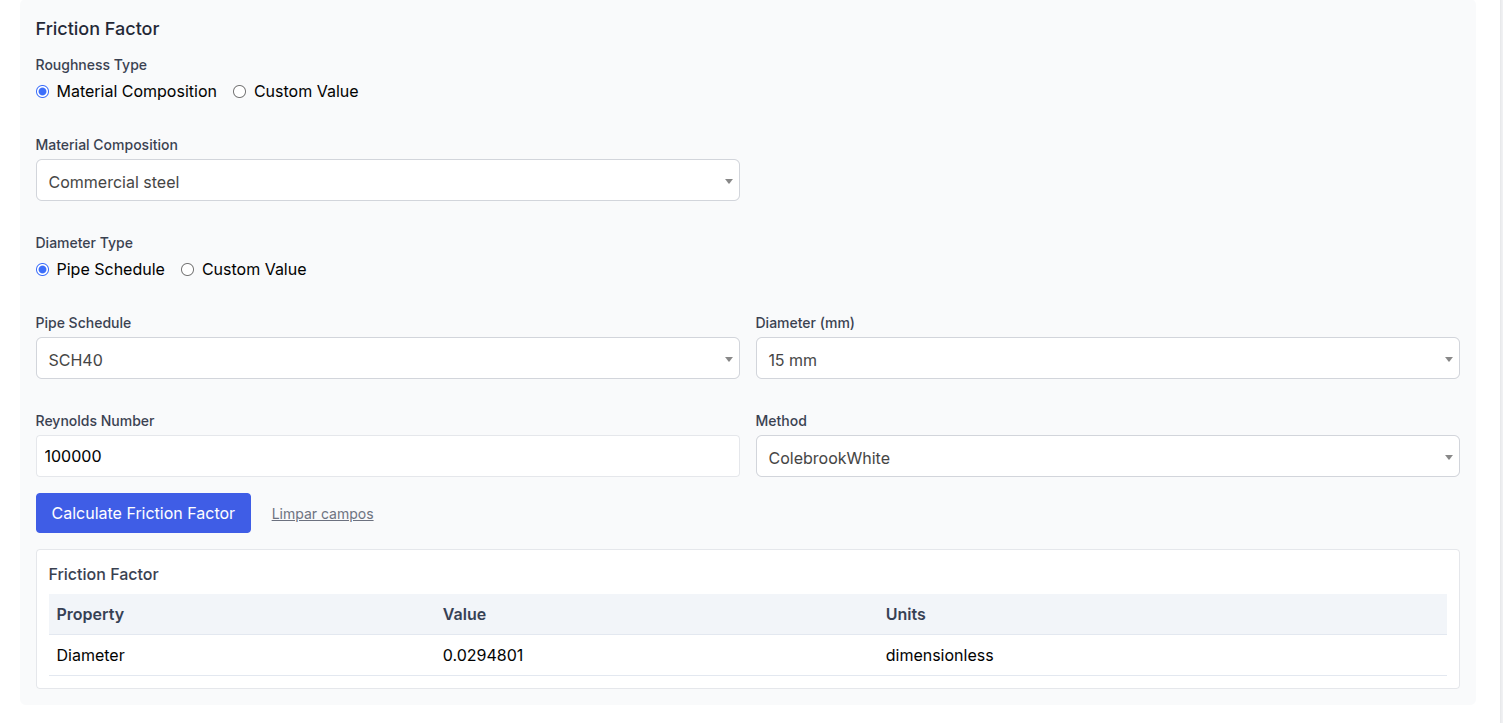
\includegraphics[width=\linewidth]{media/cap4_diagrama_moody.png}
    \fonte{Elaboração própria (2026).}
    \label{fig:friction_factor_calc}
\end{figure}

\begin{quote}
\small
\textbf{Fluxo de cálculo do fator de atrito.}
\begin{verbatim}
receber rugosidade, diâmetro, Reynolds e método
calcular rugosidade relativa
se método = ColebrookWhite, resolver a equação implicitamente
se método = SwameeJain ou Haaland, aplicar a correlação explícita
retornar fator de atrito adimensional ou erro de convergência
\end{verbatim}
\end{quote}

\subsubsection{Perda de Carga -- Darcy--Weisbach e Hazen--Williams}

A perda de carga distribuída $h_{f}$ em uma tubulação de comprimento $L$ é calculada pela equação de Darcy–Weisbach:

\begin{equation}
h_{f} = f \cdot \frac{\left( L + \sum_{}^{} L_{e q} \right)}{D} \frac{V^{2}}{2 g}
\label{eq:darcy}
\end{equation}

Na Equação \ref{eq:darcy}, $h_f$, $L$, $\sum L_{eq}$ e $D$ usam unidades de comprimento coerentes; $V$ é velocidade, por exemplo $\mathrm{m/s}$; $g$ é aceleração, por exemplo $\mathrm{m/s^2}$; e $f$ é adimensional. O resultado de $h_f$ é uma altura de perda de carga, usualmente expressa em $\mathrm{m}$. Essa fórmula é universal e independe do fluido, desde que $f$ seja adequadamente determinado \cite{perry2007}.

Para escoamento de água em tubulações de diâmetro moderado (tipicamente $D > 50\ \mathrm{mm}$) e regime turbulento plenamente estabelecido, a fórmula empírica de Hazen--Williams pode ser empregada como simplificação:

\begin{equation}
h_{f} = \frac{4{,}73 L}{C^{1{,}852}D^{4{,}87}} Q^{1{,}852}
\label{eq:hazen}
\end{equation}

Na forma exibida, o coeficiente empírico $4{,}73$ corresponde à convenção inglesa usual da correlação, com $h_f$ e $L$ em pés, $Q$ em $\mathrm{ft^3/s}$ e $D$ em pés; portanto, as unidades devem seguir a convenção associada ao coeficiente. Quando se usa a forma SI, com $h_f$ e $L$ em $\mathrm{m}$, $Q$ em $\mathrm{m^3/s}$ e $D$ em $\mathrm{m}$, o coeficiente empírico muda. Em ambas as formas, $C$ é o coeficiente de Hazen--Williams do material, tratado como adimensional e tabelado para tubulações novas de ferro fundido, aço, PVC etc. Apesar de não possuir fundamentação teórica geral, essa equação fornece boa precisão para água a 20\,°C em tubulações de transporte e é consagrada no projeto de redes de água devido à sua simplicidade \cite{perry2007,white2018}.

\begin{quote}
\small
\textbf{Fluxo de cálculo da perda de carga.}
\begin{verbatim}
receber método, geometria, vazão ou velocidade e propriedades da tubulação
resolver a velocidade ou a vazão faltante quando necessário
somar comprimento reto e comprimentos equivalentes
aplicar Darcy-Weisbach ou Hazen-Williams
retornar perda de carga em metros e validar sinal e faixa de aplicação
\end{verbatim}
\end{quote}


\subsubsection{Diâmetro Hidráulico para Geometrias Diversas}

O conceito de diâmetro hidráulico generaliza o cálculo do número de Reynolds e do fator de atrito para seções transversais não circulares. O diâmetro hidráulico é definido como:
\begin{equation}
D_{h} = \frac{4 A}{P}
\label{eq:diametro_hidraulico}
\end{equation}
onde $A$ é a área da seção transversal de escoamento e $P$ o perímetro molhado (contorno em contato com o fluido). Assim:

Para dutos circulares, conforme a Equação \ref{eq:dh_circular}:
\begin{equation}
D_{h} = D
\label{eq:dh_circular}
\end{equation}
(recupera o diâmetro interno). Para canais ou abertos, conforme a Equação \ref{eq:dh_rect}:
\begin{equation}
D_{h} = \frac{4 a b}{2 ( a + b )}
\label{eq:dh_rect}
\end{equation}
onde $a$ e $b$ são os lados do retângulo. Para anulares (espaço entre dois tubos concêntricos), conforme a Equação \ref{eq:dh_annular}:
\begin{equation}
D_{h} = D_{o} - D_{i}
\label{eq:dh_annular}
\end{equation}
(diferença entre diâmetro externo interno e diâmetro externo do interno). Para seções triangulares (por ex., condutos abertos triangulares), calcula-se $A$ e $P$ conforme a geometria e aplica-se $4 A / P$. Para geometrias mais complexas (ex.: calhas semicirculares), também se aplica $4 A / P$ considerando o perímetro molhado adequadamente.

Nas Equações \ref{eq:diametro_hidraulico} a \ref{eq:dh_annular}, $D_h$, $D$, $D_o$, $D_i$, $a$, $b$ e o perímetro molhado $P$ (ou $P_m$) usam a mesma unidade de comprimento; $A$ usa a unidade de área correspondente; e cada fórmula retorna $D_h$ nessa unidade de comprimento.

\begin{figure}[H]
    \centering
    \caption{Tipos de dutos de escoamento}
    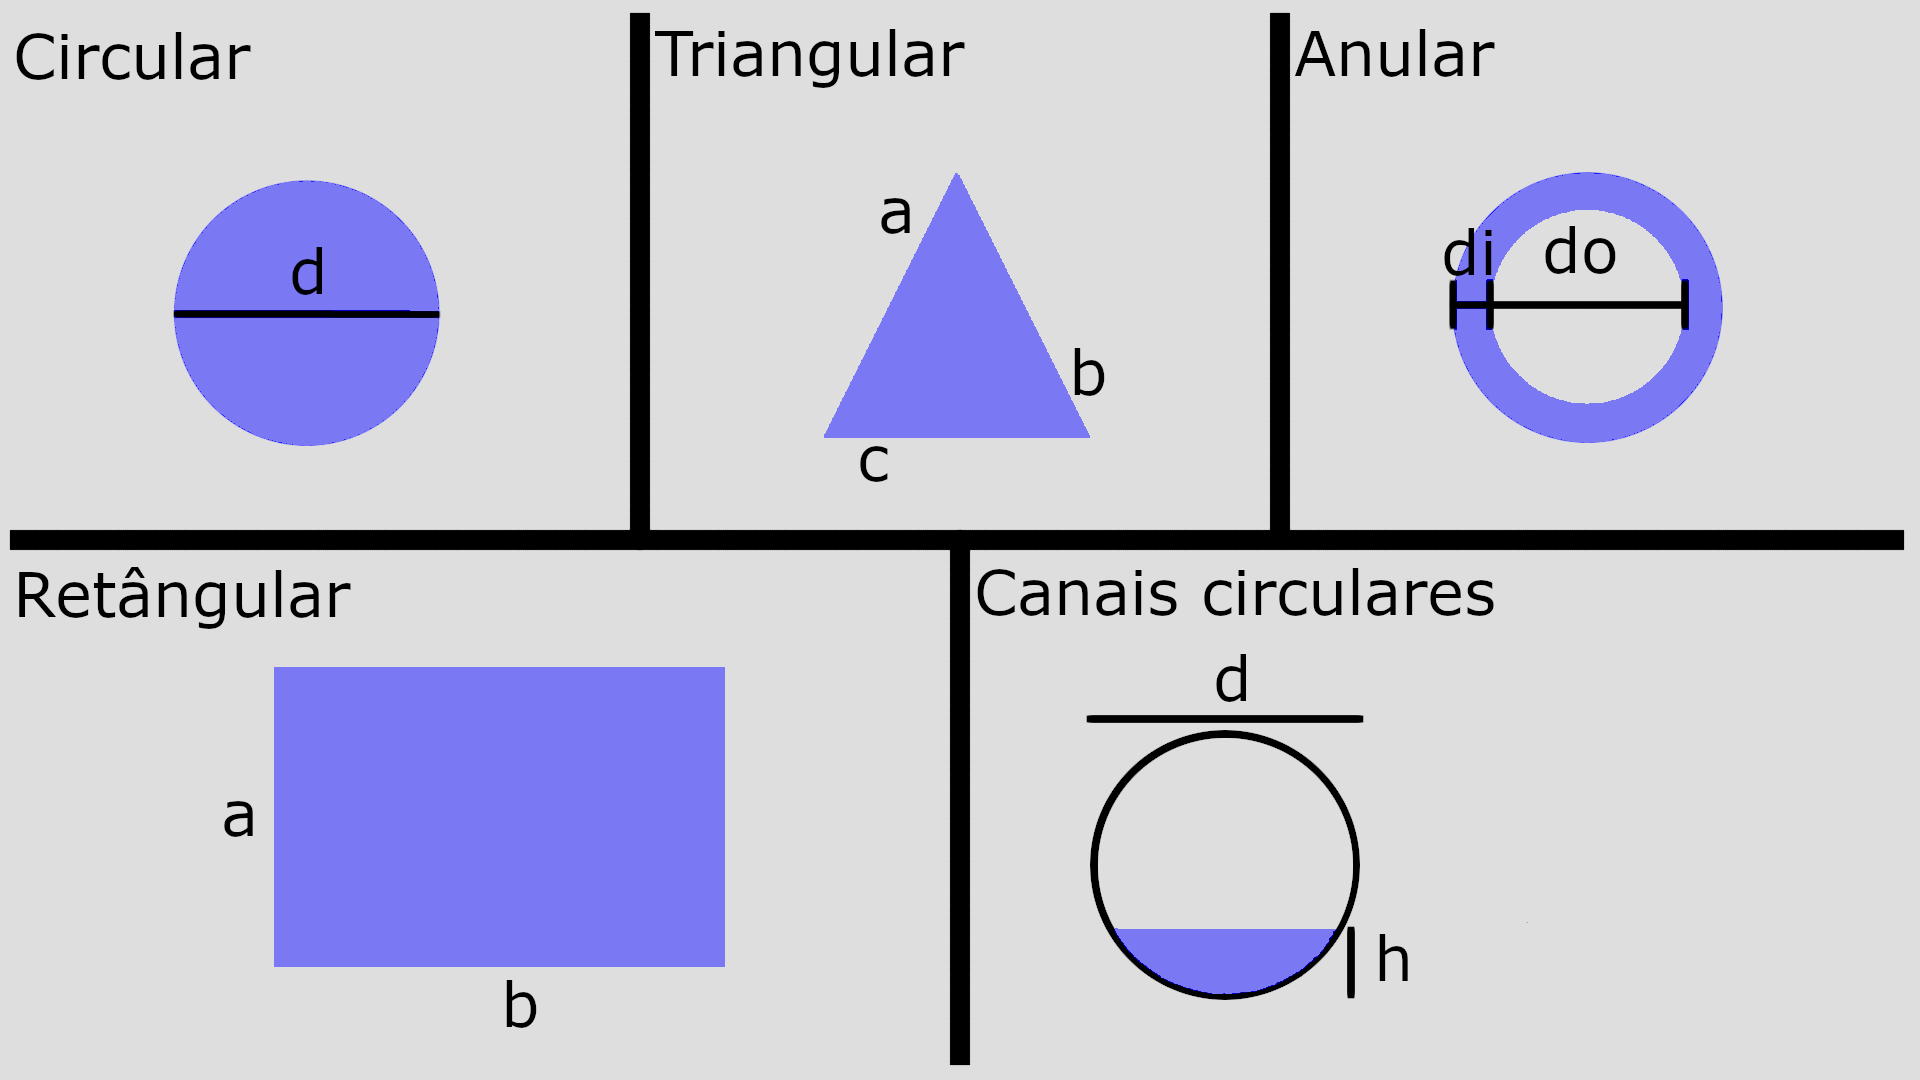
\includegraphics[width=\linewidth]{media/cap4_tipos_dutos_escoamento.png}
    \fonte{Elaboração própria (2026).}
\end{figure}

O programa permite ao usuário informar $A$ e $P$ para cálculo de $D_{h}$ em situações especiais, garantindo flexibilidade para tratar geometrias arbitrárias \cite{white2018}.

\begin{quote}
\small
\textbf{Fluxo de cálculo do diâmetro hidráulico.}
\begin{verbatim}
receber geometria e dimensões específicas da seção
calcular área e perímetro molhado conforme a geometria
aplicar Dh = 4 * área / perímetro
validar dimensões, desigualdade triangular ou altura do segmento
retornar diâmetro hidráulico na unidade de entrada
\end{verbatim}
\end{quote}

\subsection{Bombas}

\subsubsection{Altura Manométrica entre Dois Pontos}

A forma estendida da equação de Bernoulli é utilizada para avaliar as variações de carga (energia por unidade de peso do fluido) entre dois pontos de um duto de escoamento, incluindo perdas:

\begin{equation}
H = \frac{P_{2} - P_{1}}{\rho g} + \frac{V_{2}^{2} - V_{1}^{2}}{2 g} + z_{2} - z_{1} + h_f
\label{eq:bernoulli}
\end{equation}

Em que $H$ é a altura manométrica adicionada (se positiva) ou removida (se negativa) entre os pontos 1 e 2. Todos os termos da Equação \ref{eq:bernoulli} são expressos como carga hidráulica em metros: as pressões $P_1$ e $P_2$ usam unidades coerentes com $\rho$ e $g$ no termo $\frac{P_{2} - P_{1}}{\rho g}$; as velocidades $V_1$ e $V_2$ entram em $\mathrm{m/s}$; as cotas $z_1$ e $z_2$ são dadas em $\mathrm{m}$; e $h_f$ reúne as perdas distribuídas e localizadas em $\mathrm{m}$. Com essa convenção, perdas positivas aumentam a altura requerida pela bomba \cite{white2018}.

Essa equação é fundamental para avaliar a necessidade de bombeamento: uma bomba deve fornecer uma $H$ suficiente para superar as perdas e elevar o fluido da condição 1 até 2; inversamente, uma turbomáquina geradora extrairá essa energia do fluido.

\begin{figure}[H]
    \centering
    \caption{Cálculo da altura manométrica – Parte 1/2}
    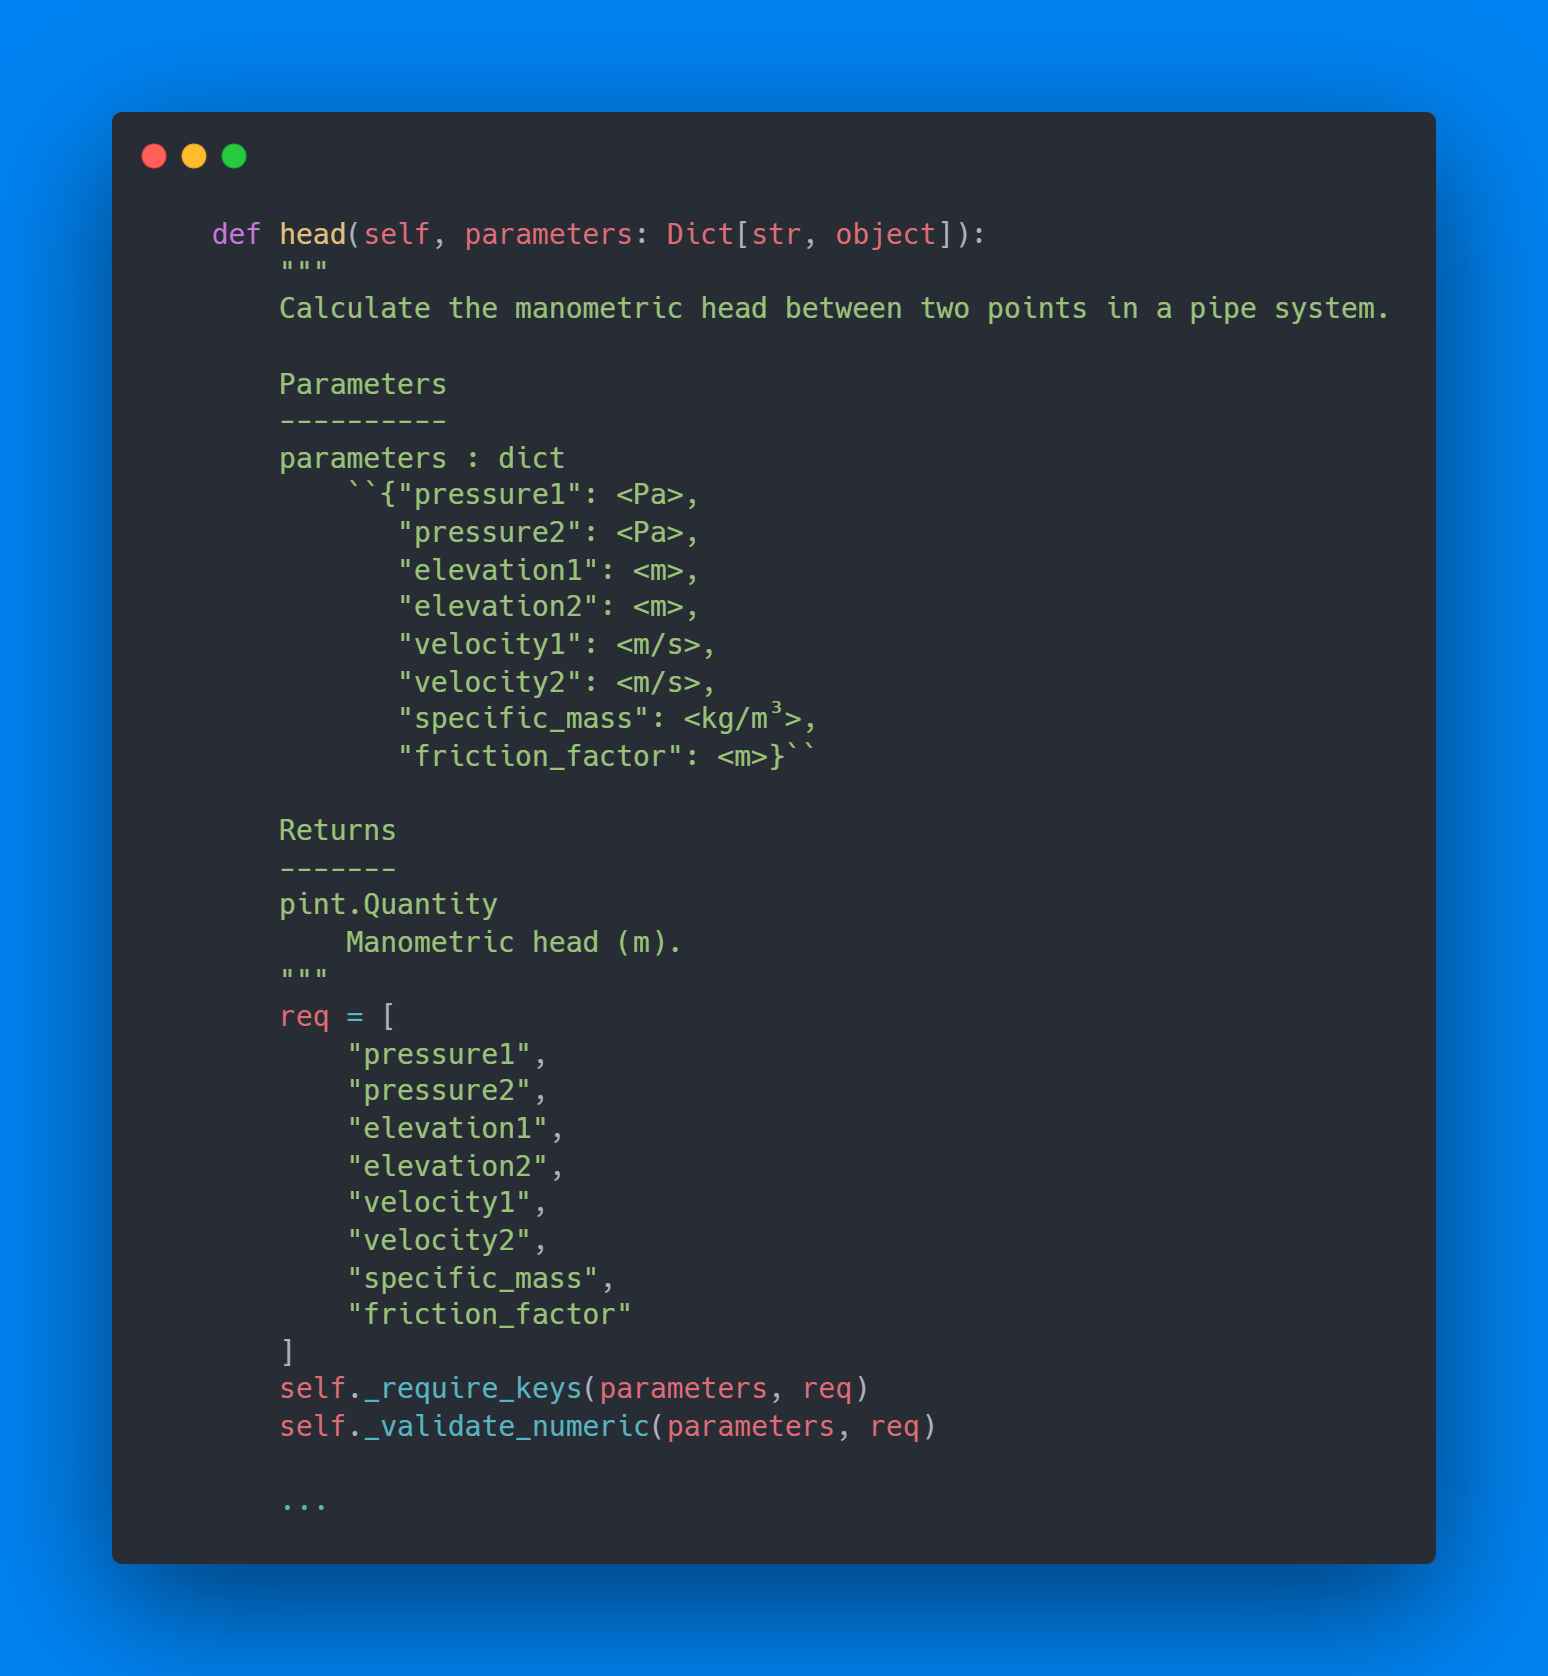
\includegraphics[width=\linewidth]{media/cap4_head_parte_um.png}
    \fonte{Elaboração própria (2026).}
\end{figure}
\begin{figure}[H]
    \centering
    \caption{Cálculo da altura manométrica – Parte 2/2}
    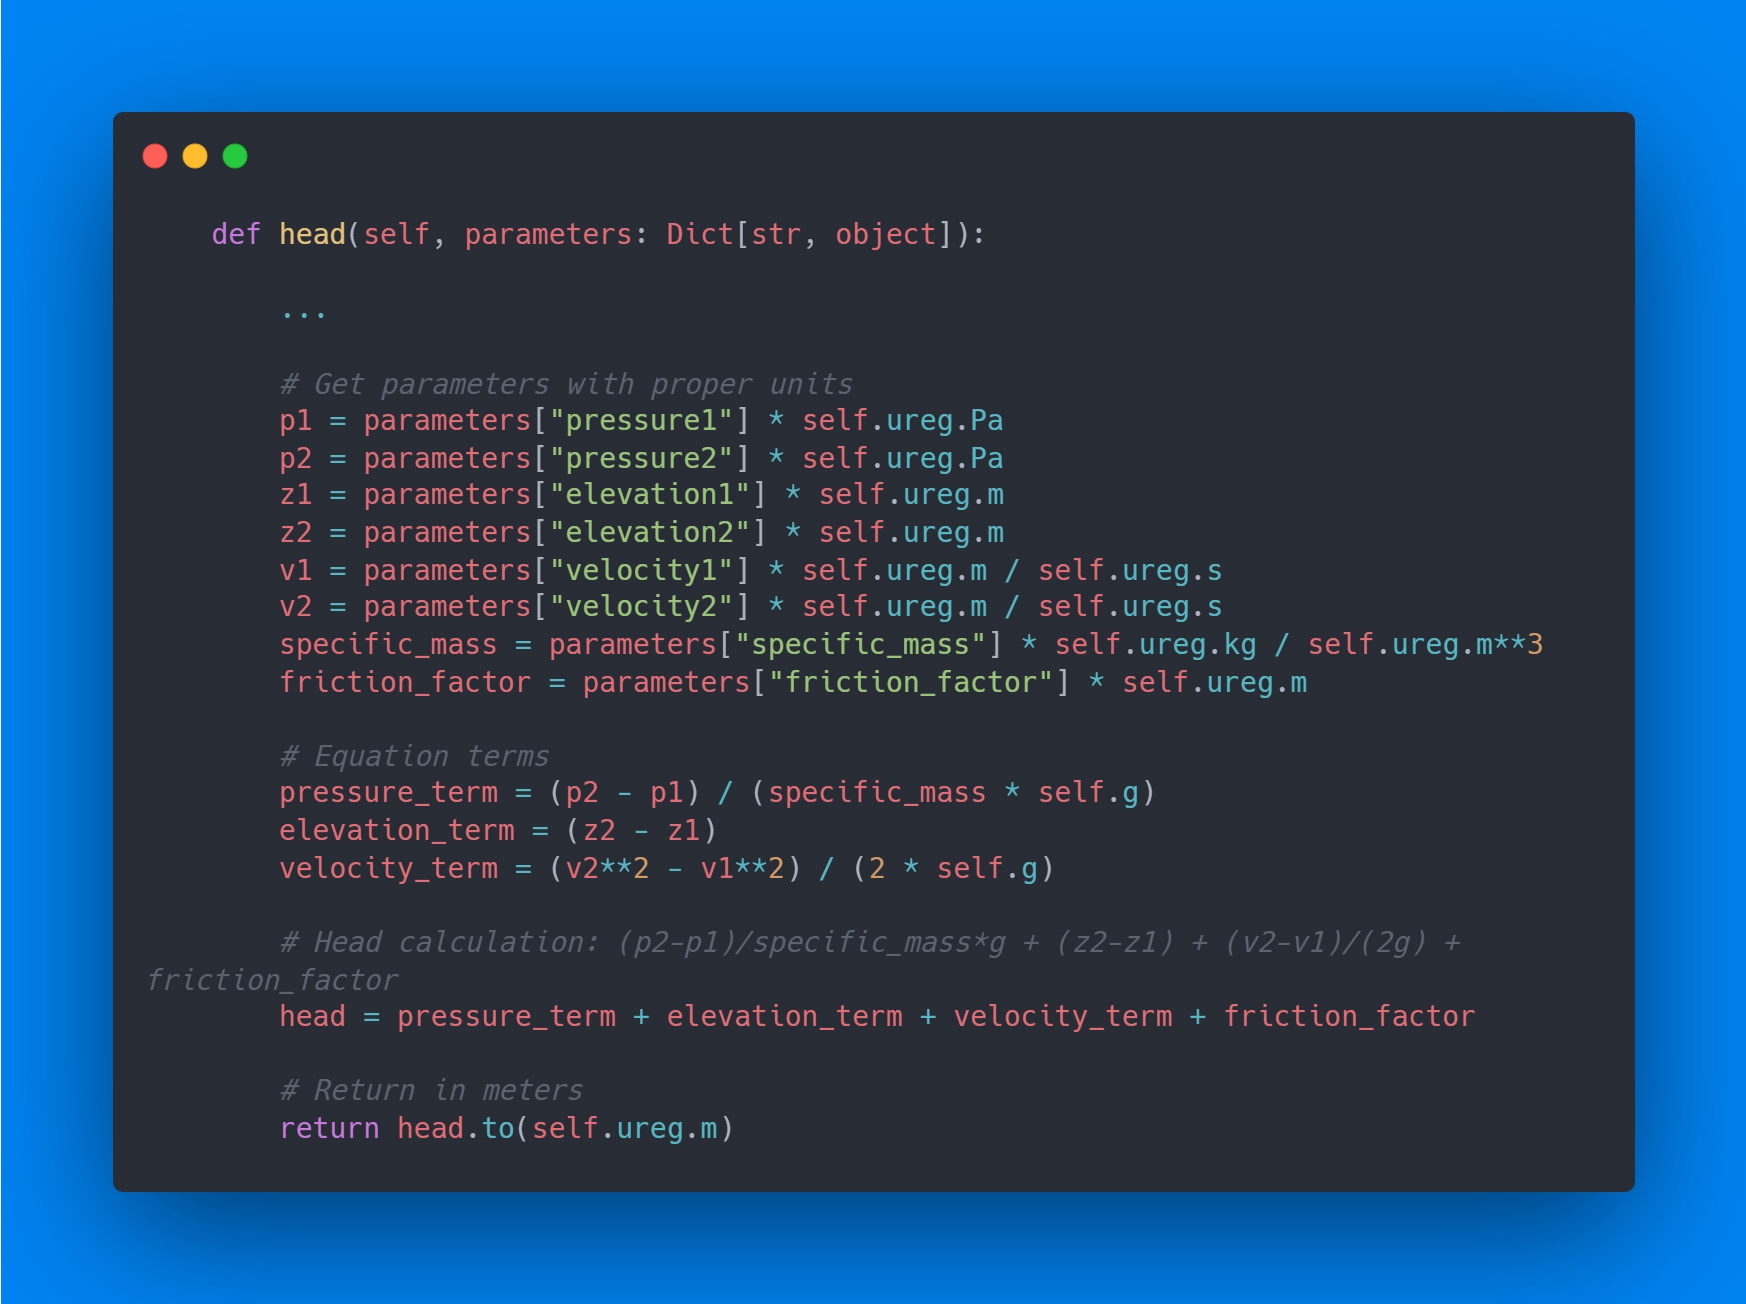
\includegraphics[width=\linewidth]{media/cap4_head_parte_dois.png}
    \fonte{Elaboração própria (2026).}
\end{figure}

\subsubsection{\textit{NPSH} Disponível}

Para evitar cavitação em bombas, calcula-se o \textit{NPSH} disponível na sucção, que deve exceder o \textit{NPSH} requerido pelo fabricante. A expressão para o \textit{NPSH} disponível, em termos de altura de líquido, é:

\begin{equation}
N P S H_{d i s p} = \frac{P_{s u c} + P_{a t m} - p_{v a p}}{\rho g} + \frac{V_{s u c}^{2} \ }{2 g} + \left( z_{s u c} - z_{0} \right) - h_{s u c}
\label{eq:npsh}
\end{equation}

O resultado da Equação \ref{eq:npsh} é expresso em metros de coluna do líquido bombeado. As pressões $P_{suc}$, $P_{atm}$ e $p_{vap}$ devem ser coerentes entre si e com $\rho g$; $\rho$ é massa específica, por exemplo $\mathrm{kg/m^3}$; $V_{suc}$ é velocidade em $\mathrm{m/s}$; $z_{suc}$ e $z_0$ são cotas em $\mathrm{m}$; e $h_{suc}$ representa as perdas na linha de sucção em $\mathrm{m}$ \cite{perry2007}.

O cálculo de \textit{NPSH} disponível permite verificar se há margem de segurança sobre o \textit{NPSH} requerido da bomba (fornecido pelo fabricante para aquela vazão), garantindo que o líquido não vaporize na entrada da bomba – o que causaria cavitação, danos e redução de desempenho.

\begin{figure}[H]
    \centering
    \caption{Cálculo do \textit{NPSH} – Parte 1/2}
    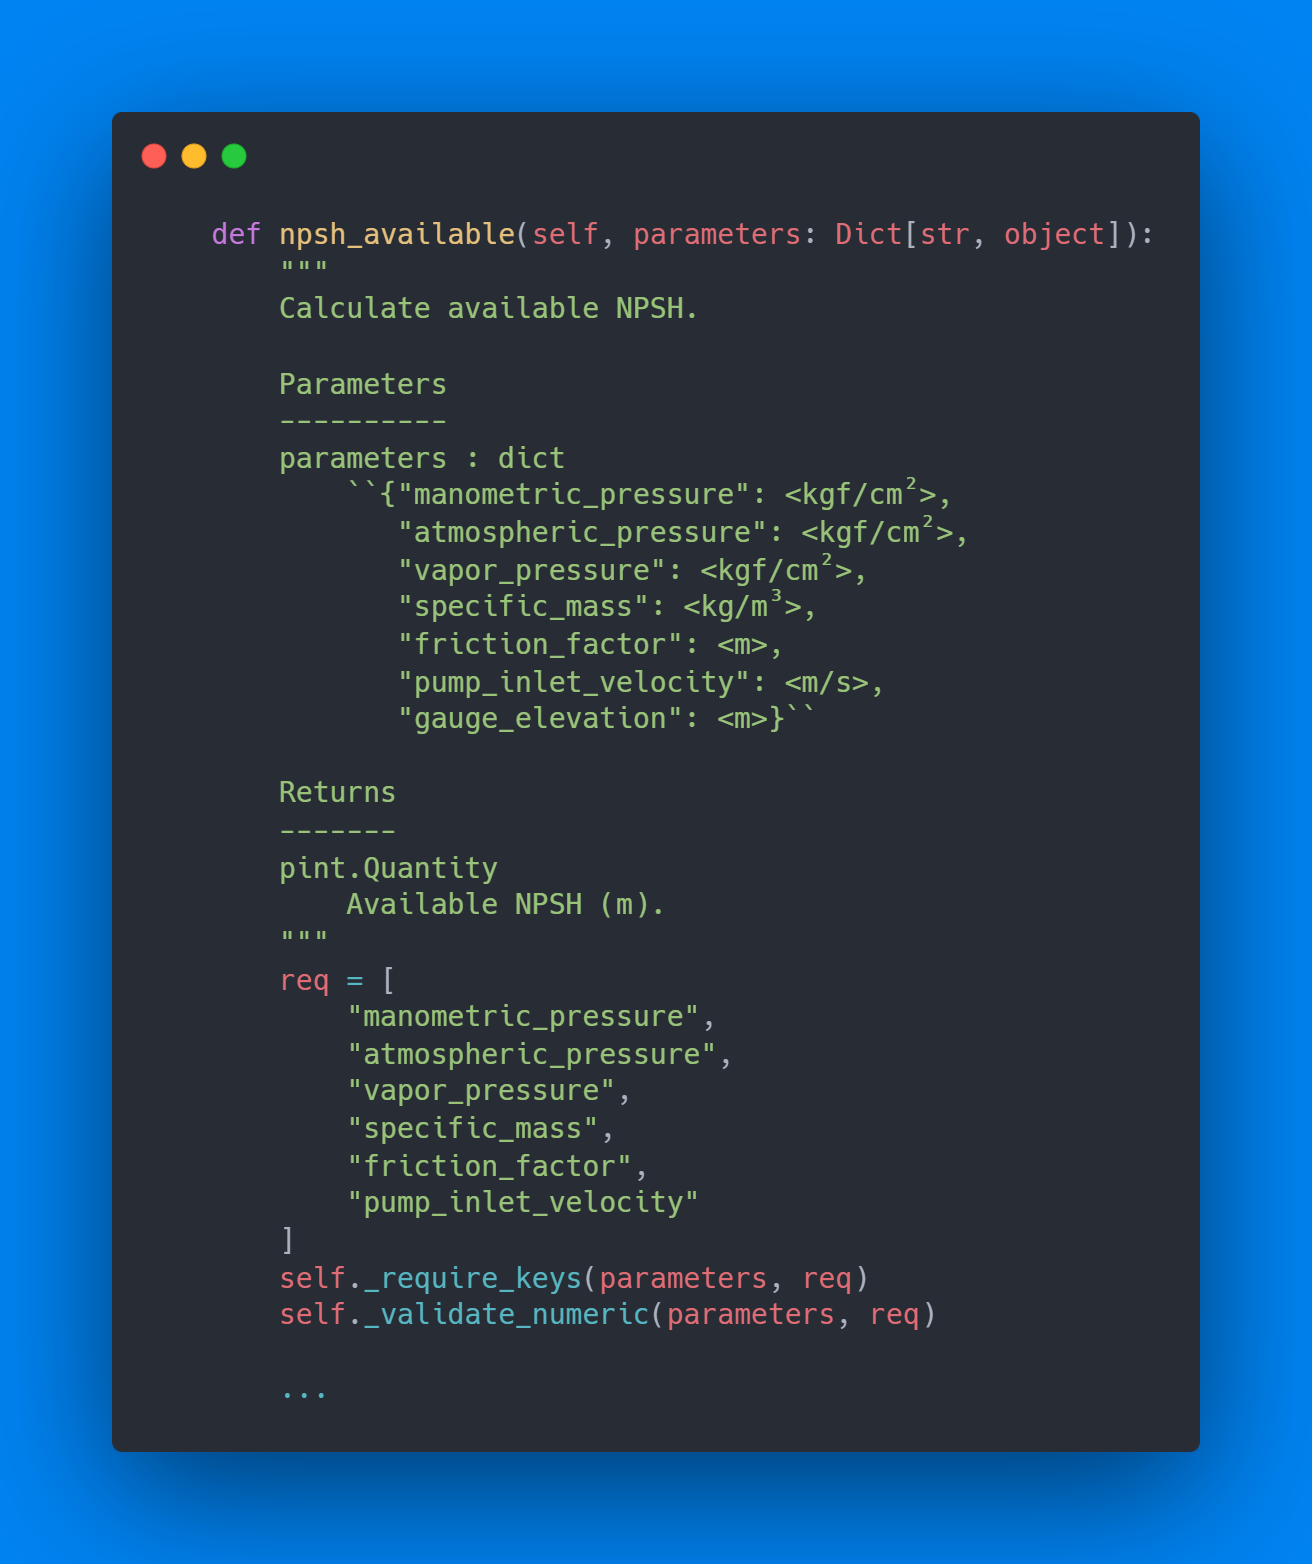
\includegraphics[width=\linewidth]{media/cap4_npsh_parte_um.png}
    \fonte{Elaboração própria (2026).}
\end{figure}

\begin{figure}[H]
    \centering
    \caption{Cálculo do \textit{NPSH} – Parte 2/2}
    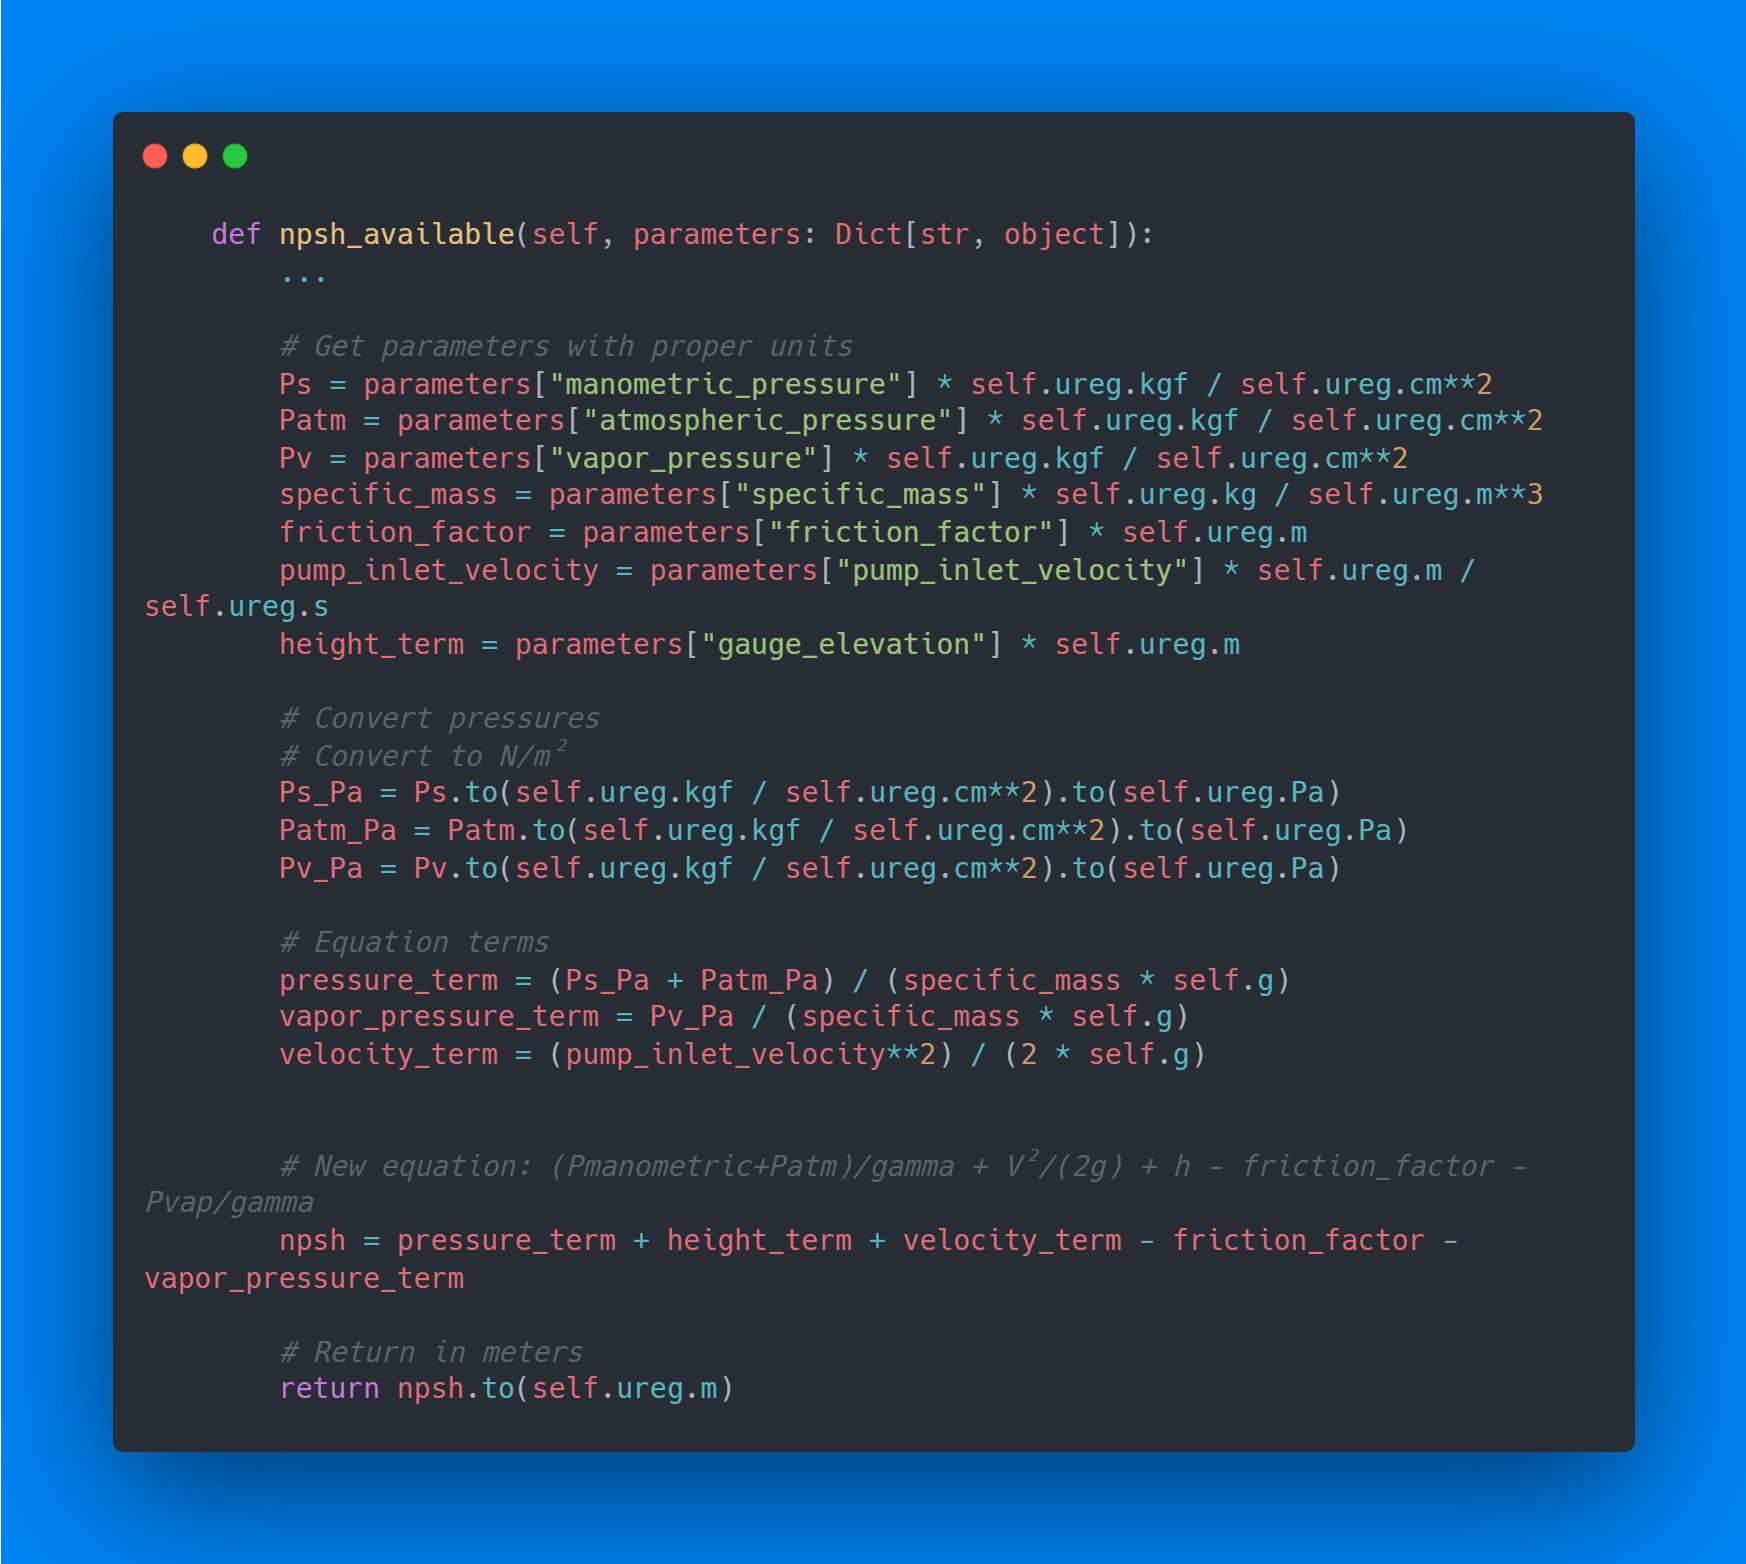
\includegraphics[width=\linewidth]{media/cap4_npsh_parte_dois.png}
    \fonte{Elaboração própria (2026).}
\end{figure}

\subsection{Propriedades Termofísicas}

Propriedades termofísicas – como massa específica, viscosidade, calor específico, condutividade térmica, entalpia e entropia – são insumos essenciais em praticamente todos os cálculos de processos. Em misturas, a predição de propriedades requer modelos mais complexos do que simples somas ponderadas, considerando interações moleculares e desvios da idealidade. Tais propriedades alimentam balanços de massa e energia, o dimensionamento térmico de trocadores, o cálculo de Reynolds e de fatores de atrito, o desempenho de separações, entre outros. Temperatura e pressão são variáveis determinantes: utilizam-se correlações empíricas (por exemplo, equação de Antoine para pressão de vapor) ou equações de estado (gás ideal, Peng-Robinson, SRK) conforme o sistema. Erros na estimativa de viscosidade ou massa específica afetam o cálculo de Reynolds, fator de atrito e potência de bombeamento; imprecisões em calores específicos ou entalpias propagam-se em balanços de energia e projeto de utilidades.

\begin{table}[H]
    \centering
    \caption{Fluxo de obtenção de propriedades termofísicas}
    \label{tab:fluxo-propriedades-termofisicas}
    \small
    \begin{tabular}{p{0.25\textwidth}p{0.57\textwidth}}
        \hline
        \textbf{Etapa} & \textbf{Descrição} \\
        \hline
        Entradas & Fluido, propriedade solicitada, temperatura em K e pressão em Pa; para propriedades críticas, apenas o fluido. \\
        Processamento & Consulta \textit{CoolProp}, trata propriedades de saturação e associa unidades SI por meio do \textit{Pint}. \\
        Saída & Propriedade solicitada ou conjunto de propriedades, incluindo propriedades críticas quando aplicável. \\
        Validação & Confere a existência do fluido e comunica falhas de consulta ou propriedades indisponíveis. \\
        \hline
    \end{tabular}
    \fonte{Autoria própria.}
\end{table}

No \textit{software} desenvolvido, um módulo de propriedades utiliza a biblioteca \textit{CoolProp} para recuperar propriedades de fluidos puros (e misturas) a partir de dados de entrada de $T$ e $P$. São obtidas propriedades como massa específica ($\rho$), viscosidade, calor específico ($c_{p}$ e $c_{v}$), condutividade térmica, entalpia, entropia, massa molar e tensão superficial, além de propriedades críticas e pontos de saturação (bolha/orvalho) quando aplicável. A visualização desse cálculo de propriedades, com foco no resultado para uma mistura, é apresentada na Figura \ref{fig:mixture_properties}.

\begin{figure}[H]
    \centering
    \caption{Interface de cálculo para as propriedades de uma mistura}
    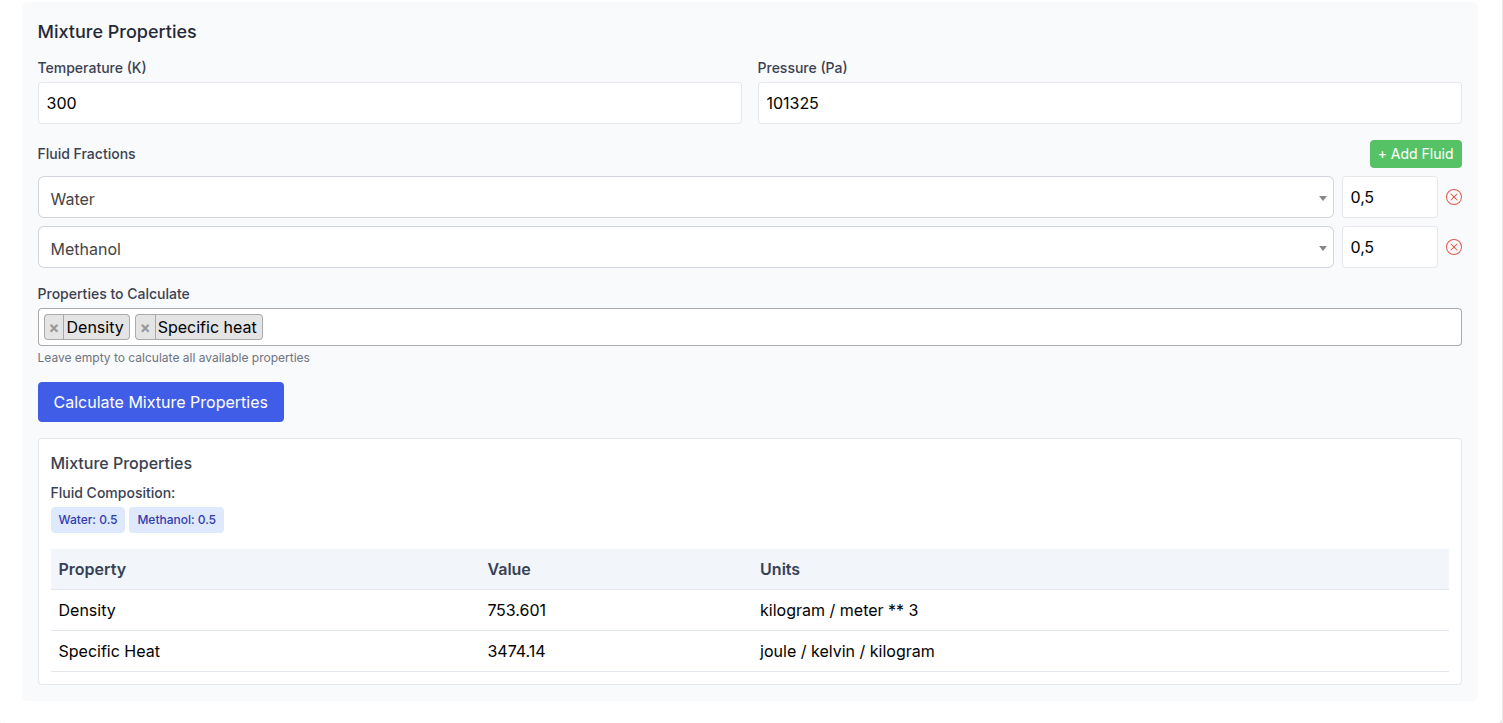
\includegraphics[width=\linewidth]{media/cap4_interface_propriedades_mistura.png}
    \fonte{Elaboração própria (2026).}
    \label{fig:mixture_properties}
\end{figure}

Para misturas, a \textit{API} do \textit{CoolProp} permite montar \textit{strings} com o padrão abaixo, usando as frações especificadas para cada componente \cite{bell2014}:

\begin{quote}
\small\texttt{HEOS::Comp1[x1]\&Comp2[x2]\&...}
\end{quote}

Todas as grandezas retornam já associadas a unidades do SI (via integração com a biblioteca \textit{Pint}), garantindo consistência nos cálculos.

\begin{table}[H]
    \centering
    \caption{Fluxo de obtenção de propriedades de misturas}
    \label{tab:fluxo-propriedades-misturas}
    \small
    \begin{tabular}{p{0.25\textwidth}p{0.57\textwidth}}
        \hline
        \textbf{Etapa} & \textbf{Descrição} \\
        \hline
        Entradas & Frações dos componentes, temperatura, pressão e, opcionalmente, a lista de propriedades. \\
        Preparação & Verifica os componentes, confere se as frações somam aproximadamente uma unidade e monta a representação da mistura. \\
        Processamento & Consulta as propriedades selecionadas na \textit{API} do \textit{CoolProp} usando a composição informada. \\
        Saída e validação & Retorna um conjunto de propriedades com unidades SI e rejeita componentes desconhecidos ou frações incompatíveis. \\
        \hline
    \end{tabular}
    \fonte{Autoria própria.}
\end{table}

O uso de uma biblioteca de propriedades de qualidade referência como o \textit{CoolProp} assegura que o \textit{software} tenha um \textit{backend} termodinâmico rigoroso e abrangente, reforçando o caráter didático ao permitir explorar diferentes cenários com fidelidade física.

\subsection{Reatores}

Reatores são equipamentos projetados para promover reações químicas, convertendo reagentes em produtos sob condições controladas de operação.

Modelos ideais como \textit{CSTR}, \textit{PFR} e batelada fornecem limites úteis para projeto e análise de desempenho. As variáveis centrais envolvidas no projeto de reatores incluem conversão dos reagentes, seletividade e rendimento (em caso de múltiplas reações), velocidade de reação, tempo de residência, volume do reator e condições de operação (temperatura, pressão). Industrialmente, o correto dimensionamento de reatores afeta diretamente a capacidade produtiva, a qualidade do produto e a segurança, especialmente no controle de remoção de calor em reações exotérmicas. A cinética química depende fortemente da temperatura (lei de Arrhenius) e da forma funcional da taxa de reação (ordem de reação, efeitos de inibição, presença de inertes, variação volumétrica em fase gasosa etc.). Erros na previsão de conversão ou no cálculo do volume reacional podem levar a baixa seletividade, formação de pontos quentes (\textit{hot spots}) e riscos operacionais. A base teórica conjuga balanços de massa por componente com leis cinéticas apropriadas, integradas no espaço (\textit{PFR}) ou no tempo de residência (\textit{CSTR}), podendo incluir balanço de energia quando o regime térmico é relevante \cite{fogler2009,levenspiel2000}.

No escopo deste projeto, são considerados reatores isotérmicos e monofásicos (todos os reagentes e produtos em uma única fase, líquida ou gasosa). O código rejeita misturas de componentes em estados físicos diferentes, a fim de garantir a validade dos balanços e do coeficiente de variação volumétrica utilizado para o estado atual dos módulos de cálculo para reatores.

A Tabela \ref{tab:unidades-reatores-estequiometria} padroniza a leitura dimensional das Equações \ref{eq:razao_reagente} a \ref{eq:dilution_factor}. Assim, os parágrafos seguintes se concentram no papel físico de cada relação.

\begin{table}[H]
    \centering
    \caption{Unidades e natureza dos símbolos nas relações estequiométricas e cinéticas de reatores}
    \label{tab:unidades-reatores-estequiometria}
    \begin{tabular}{|p{0.30\textwidth}|p{0.60\textwidth}|}
        \hline
        \textbf{Símbolo} & \textbf{Unidade ou natureza} \\ \hline
        $N_{i0}$ & Vazão molar, por exemplo $\mathrm{mol/s}$. \\ \hline
        $\nu_i$, $\nu_A$, $\nu_P$, $\nu_R$ & Coeficientes estequiométricos adimensionais. \\ \hline
        $C_i$, $C_{i0}$, $C_{A0}$ & Concentração molar, por exemplo $\mathrm{mol/m^3}$. \\ \hline
        $X$ & Conversão adimensional. \\ \hline
        $y_{A0}$ & Fração molar adimensional do reagente limitante na alimentação. \\ \hline
        $\varepsilon$ & Coeficiente de variação volumétrica adimensional. \\ \hline
        $\psi$ & Fator de diluição adimensional. \\ \hline
        $P$, $P_0$ & Pressões em unidades coerentes entre si, usadas apenas na razão $P_0/P$. \\ \hline
        $T$, $T_0$ & Temperaturas absolutas em $\mathrm{K}$, usadas apenas na razão $T/T_0$. \\ \hline
        $r$ ou $-r_A$ & Taxa molar de reação por volume de reator, por exemplo $\mathrm{mol/(m^3\,s)}$. \\ \hline
        $k$ & Constante cinética com unidades definidas pela ordem global da reação. \\ \hline
    \end{tabular}
\end{table}

Algumas lógicas gerais se aplicam a todos os tipos de reatores implementados. Por exemplo, a determinação do reagente limitante identifica o reagente cuja disponibilidade inicial por unidade estequiométrica é a menor entre os reagentes presentes. Em termos de cálculo, percorrem-se apenas os reagentes (coeficientes estequiométricos negativos), calculando conforme a Equação \ref{eq:razao_reagente}:
\begin{equation}
\mathrm{razao}_{i} = \frac{N_{i0}}{|\nu_i|}
\label{eq:razao_reagente}
\end{equation}
O quociente compara a disponibilidade molar de cada reagente por unidade estequiométrica. O valor absoluto $|\nu_i|$ evita a inversão de sinal causada pela convenção negativa dos reagentes; o reagente com menor valor de $\mathrm{razao}_{i}$ é o limitante \cite{felder2005}.

\begin{quote}
\small
\textbf{Pseudocódigo da preparação estequiométrica do reator.}
\begin{verbatim}
identificar reagentes com coeficiente estequiometrico negativo
calcular disponibilidade molar normalizada de cada reagente
selecionar o menor valor normalizado como reagente limitante
calcular fator de diluicao a partir de conversao, pressao e temperatura
atualizar concentracoes de saida por estequiometria
calcular velocidade de reacao pela lei cinetica informada
\end{verbatim}
\end{quote}

A velocidade de reação é modelada, em geral, por uma lei de potência do tipo:

\begin{equation}
r = k \cdot \prod_{}^{} C_{i}^{n_{i}}
\label{eq:rate_law}
\end{equation}

A Equação \ref{eq:rate_law} representa uma lei de potência: cada concentração entra elevada à sua ordem de velocidade, e $k$ assume a unidade necessária para que o produto resulte em taxa volumétrica de reação.

A integração da cinética com a estequiometria é feita via conversão $X$ do reagente limitante. Os balanços estequiométricos relacionam as concentrações de saída de cada componente à conversão $X$. Para cada componente $i$ na reação, tem-se a seguinte relação geral: o termo estequiométrico é positivo para formação (produtos), negativo para consumo (reagentes) e nulo para inertes.

\begin{equation}
C_{i} = \frac{C_{i0} + \left( \frac{\nu_i}{|\nu_A|} \cdot C_{A0} \cdot X \right)}{\psi}
\label{eq:conc_stoich}
\end{equation}

A Equação \ref{eq:conc_stoich} ajusta a concentração de cada componente pela conversão do reagente limitante. O numerador representa consumo ou formação estequiométrica, enquanto o denominador aplica a diluição total do meio.

Para determinação do coeficiente de variação volumétrica para reações gasosas, a Equação \ref{eq:epsilon_def} deve ser utilizada.

\begin{equation}
\varepsilon = y_{A0} \cdot \frac{\sum_{\nu_i>0} \nu_i - \sum_{\nu_i<0} |\nu_i|}{|\nu_{A}|}
\label{eq:epsilon_def}
\end{equation}

O numerador compara a quantidade estequiométrica formada e consumida na fase gasosa, normalizada pelo reagente limitante. O sinal de $\varepsilon$ indica expansão ou contração molar associada à reação.

\begin{equation}
\psi = ( 1 + \varepsilon X ) \frac{P_{0}}{P} \frac{T}{T_{0}}
\label{eq:dilution_factor}
\end{equation}

Onde $\varepsilon$ representa a variação volumétrica ou molar por mol de $A$ reagido, podendo indicar expansão ou contração conforme a estequiometria e a fase gasosa. O fator $\psi$ agrega a variação volumétrica estequiométrica (via $\varepsilon X$) e as correções de pressão e temperatura em relação às condições iniciais \cite{levenspiel2000}. Essas relações estequiométricas permitem calcular as concentrações de saída de todos os componentes a partir da conversão $X$ do reagente limitante, sendo a base para os balanços nos diferentes modelos de reatores.

\subsubsection{Reator do Tipo \textit{CSTR}}

O reator do tipo \textit{CSTR} é um tanque agitado operando em regime contínuo. Assume-se mistura completa no interior do tanque (composição uniforme em todo o volume). A conversão é desenvolvida integralmente dentro do volume do reator, dependendo do balanço entre a cinética de reação e o tempo de residência dos reagentes no tanque.

No sistema implementado, são suportados três casos de uso: (i) conversão desejada e cinética conhecidas (calcula-se o volume do reator necessário), (ii) volume disponível e cinética conhecidas (calcula-se a conversão atingida) e (iii) tempo de residência e cinética conhecidos (calcula-se a conversão atingida). As saídas calculadas pelo algoritmo incluem, entre outros: conversão do reagente limitante $X$, vazão molar do reagente limitante na entrada $F_{A0}$, vazão volumétrica total na saída $Q_{T}$, volume do reator $V$, taxa de reação $r$ no interior, concentrações de saída $C_{i,\mathrm{saida}}$, fator de diluição $\psi$, coeficiente de variação volumétrica $\varepsilon$ e tempo de residência $\tau$.

A Tabela \ref{tab:unidades-cstr} resume as unidades locais da sequência de cálculo do \textit{CSTR}; essas definições valem para as Equações \ref{eq:molar_flow_in} a \ref{eq:volume_calc}.

\begin{table}[H]
    \centering
    \caption{Unidades e natureza dos símbolos na sequência de cálculo do \textit{CSTR}}
    \label{tab:unidades-cstr}
    \begin{tabular}{|p{0.30\textwidth}|p{0.60\textwidth}|}
        \hline
        \textbf{Símbolo} & \textbf{Unidade ou natureza} \\ \hline
        $N_{i0}$, $F_{A0}$ & Vazão molar, por exemplo $\mathrm{mol/s}$. \\ \hline
        $Q_i$, $Q_T$ & Vazão volumétrica, por exemplo $\mathrm{m^3/s}$. \\ \hline
        $C_{i0}$, $C_{i0e}$ & Concentração molar, por exemplo $\mathrm{mol/m^3}$. \\ \hline
        $V$ & Volume do reator, por exemplo $\mathrm{m^3}$. \\ \hline
        $X$ & Conversão adimensional. \\ \hline
        $-r_A$ & Taxa molar de reação por volume de reator, por exemplo $\mathrm{mol/(m^3\,s)}$. \\ \hline
        $\tau$ & Tempo de residência, por exemplo $\mathrm{s}$. \\ \hline
        $f(X)$ em \ref{eq:cstr_obj_function} & Resíduo objetivo: diferença numérica entre conversões adimensionais. \\ \hline
    \end{tabular}
\end{table}

\paragraph{Conversão e Cinética (Cálculo do Volume)}

Passos principais do cálculo:
\begin{itemize}
    \item Identificação do reagente limitante (conforme descrito anteriormente);
    \item Cálculo das vazões molares de entrada pela Equação \ref{eq:molar_flow_in}:
    \begin{equation}
    N_{i 0} = Q_{i} \cdot C_{i 0 e}
    \label{eq:molar_flow_in}
    \end{equation}
    para cada componente, bem como da vazão volumétrica total pela Equação \ref{eq:total_flow}:
    \begin{equation}
    Q_{T} = \sum_{}^{} Q_{i}
    \label{eq:total_flow}
    \end{equation}
    As concentrações iniciais (após mistura das correntes de alimentação) são dadas pela Equação \ref{eq:initial_conc}:
    \begin{equation}
    C_{i 0} = \frac{N_{i 0}}{Q_{T}}
    \label{eq:initial_conc}
    \end{equation}
    \item Cálculo do fator de diluição total $\psi$ com a conversão alvo $X$ (Equação \ref{eq:dilution_factor});
    \item Cálculo da taxa de reação $r$ a partir da constante cinética $k$ e das concentrações na saída (considerando $X$), supondo regime isotérmico \cite{fogler2009};
    \item Aplicação do balanço no \textit{CSTR} para o reagente limitante.
\end{itemize}

Para conversão $X$ conhecida, a equação de \textit{design} é dada por:

\begin{equation}
V = \frac{F_{A 0} \cdot X}{- r_{A}}
\label{eq:cstr_design}
\end{equation}

Nessa expressão, o produto $F_{A0}X$ representa a vazão molar convertida do reagente limitante, e a divisão pela taxa de consumo volumétrica fornece o volume requerido do tanque.

Cálculo do tempo de residência:

\begin{equation}
\tau = \frac{V}{Q_{T}}
\label{eq:residence_time}
\end{equation}

A fim de simplificar as rotinas, utiliza-se a função \textit{\_initialize\_reactor()}, que calcula as concentrações e vazões de cada componente na entrada, bem como o coeficiente de variação volumétrica ou molar, o fator de diluição, as temperaturas e pressões iniciais e finais e o reagente limitante.

\paragraph{Volume e Cinética (Cálculo da Conversão)}

Nesse caso, são conhecidos o volume do reator $V$ e a cinética (expressão da taxa $r ( C_{i} )$, incluindo $k$). Deseja-se determinar a conversão $X$ atingida no \textit{CSTR}. Isolando $X$ na equação de \textit{design} do \textit{CSTR} obtém-se uma equação implícita. Define-se então uma função objetivo:

\begin{equation}
f ( x ) = \frac{{| v}_{A} | \cdot r_{A} \cdot V}{F_{A 0}} - X
\label{eq:cstr_obj_function}
\end{equation}

Então encontra-se sua raiz na faixa 0<X<1, tipicamente utilizando o método de Brent, dada a monotonicidade esperada de $f ( x )$. A raiz X que satisfaz $f ( x ) = 0$ corresponde à conversão no reator.

\paragraph{Tempo de Residência e Cinética}

Conhecido o tempo de residência $\tau$, calcula-se inicialmente pela Equação \ref{eq:volume_calc}:
\begin{equation}
V = Q_{T} \cdot \tau
\label{eq:volume_calc}
\end{equation}
Em seguida, o problema se reduz ao caso anterior: aplica-se a mesma função objetivo $f ( X )$ da Equação \ref{eq:cstr_obj_function} e resolve-se numericamente para $X$, obtendo a conversão atingida no \textit{CSTR} com tempo de residência $\tau$ especificado.

\begin{table}[H]
    \centering
    \caption{Etapas computacionais do modelo \textit{CSTR}}
    \label{tab:metodologia-cstr-etapas}
    \small
    \begin{tabular}{p{0.28\textwidth}p{0.58\textwidth}}
        \hline
        \textbf{Etapa} & \textbf{Responsabilidade} \\
        \hline
        Inicialização & Normaliza unidades, identifica o reagente limitante e prepara as variáveis de entrada. \\
        Cálculo por conversão & Usa a conversão especificada para obter concentrações, velocidade de reação e volume requerido. \\
        Cálculo por volume & Resolve a conversão compatível com o volume informado. \\
        Cálculo por tempo de residência & Relaciona vazão, volume, tempo de residência e cinética para fechar o estado do reator. \\
        \hline
    \end{tabular}
    \fonte{Autoria própria.}
\end{table}

\subsubsection{Reator do Tipo \textit{PFR}}

Um reator tubular é caracterizado por escoamento pistonado, sem mistura axial significativa: cada elemento de fluido que entra percorre o reator como se fosse um reator batelada em movimento, evoluindo em conversão conforme o comprimento.

Para uma conversão alvo $X$, o volume requerido de um \textit{PFR} ideal é dado pela integração da equação de \textit{design} diferencial ao longo da conversão \cite{levenspiel2000}. Matematicamente:

\begin{equation}
V = {( R + 1 ) \cdot F}_{A 0} \cdot \int_{\frac{R}{R + 1} X \ }^{X} \frac{d X}{- r_{A}}
\label{eq:pfr_design}
\end{equation}

A Tabela \ref{tab:unidades-pfr} padroniza a leitura dimensional da Equação \ref{eq:pfr_design}; o texto seguinte interpreta os termos sem repetir a lista de unidades.

\begin{table}[H]
    \centering
    \caption{Unidades e natureza dos símbolos no dimensionamento do \textit{PFR}}
    \label{tab:unidades-pfr}
    \begin{tabular}{|p{0.30\textwidth}|p{0.60\textwidth}|}
        \hline
        \textbf{Símbolo} & \textbf{Unidade ou natureza} \\ \hline
        $V$ & Volume do reator, por exemplo $\mathrm{m^3}$. \\ \hline
        $F_{A0}$ & Vazão molar do reagente limitante na alimentação fresca, por exemplo $\mathrm{mol/s}$. \\ \hline
        $X$, $R$ & Conversão e razão de reciclo adimensionais. \\ \hline
        $-r_A$ & Taxa molar de reação por volume de reator, por exemplo $\mathrm{mol/(m^3\,s)}$, quando a equação é escrita em base molar. \\ \hline
    \end{tabular}
\end{table}

O termo $R$ representa a razão de reciclo ou recirculação, definida como vazão reciclada dividida pela vazão fresca de alimentação. Assim, $( R + 1 )$ acomoda o aumento da vazão que atravessa o reator na integração. No código, essa integral é avaliada numericamente (por exemplo, via \textit{scipy.integrate.quad}). Para o caso inverso, em que $V$ é conhecido e se busca $X$, utiliza-se novamente um procedimento iterativo (método de Brent) aplicando a equação de \textit{design} diferencial até encontrar a conversão cujo volume calculado corresponda ao especificado \cite{fogler2009}.

A representação gráfica dessa relação é apresentada pelos perfis de \textit{Levenspiel} do \textit{software}, que permitem interpretar a área associada ao volume requerido e comparar \textit{CSTR} e \textit{PFR}.

Considerando a similaridade estrutural e semântica com as rotinas de cálculo do \textit{CSTR}, destaca-se a diferença na função objetivo usada para o cálculo de volume, apresentada no pseudocódigo a seguir.

\begin{quote}
\small
\textbf{Pseudocódigo da integração do \textit{PFR}.}
\begin{verbatim}
definir conversao inicial e conversao alvo
para cada ponto de integracao:
    calcular concentracoes pela estequiometria
    calcular velocidade de reacao no ponto
    integrar dV/dX = F_A0 / (-r_A)
retornar volume acumulado, perfil de conversao e estados intermediarios
\end{verbatim}
\end{quote}

\subsection{Balanço de Massa}

O balanço de massa aplica o princípio da conservação da massa a sistemas de processo: em regime estacionário, a massa que entra em um sistema deve ser igual à massa que sai, ajustada pela geração ou consumo devido a reações químicas \cite{felder2005}. Para cada componente, a quantidade produzida ou consumida deve ser contabilizada segundo a estequiometria.

A Tabela \ref{tab:unidades-balanco-massa} resume a base dimensional comum das Equações \ref{eq:mass_balance_word} a \ref{eq:gross_product_flow}. A mesma base deve ser mantida dentro de cada balanço.

\begin{table}[H]
    \centering
    \caption{Unidades e natureza dos termos no balanço de massa com reciclo}
    \label{tab:unidades-balanco-massa}
    \begin{tabular}{|p{0.30\textwidth}|p{0.60\textwidth}|}
        \hline
        \textbf{Símbolo ou termo} & \textbf{Unidade ou natureza} \\ \hline
        Acúmulo, entradas, saídas, geração e consumo & Mesma base escolhida para o balanço por tempo, como $\mathrm{kg/s}$ ou $\mathrm{mol/s}$. \\ \hline
        $\dot{m}$ & Vazão mássica, por exemplo $\mathrm{kg/s}$. \\ \hline
        $F_R$, $F_G$, $F_P$ & Vazões na mesma base selecionada para o balanço: molar, mássica ou volumétrica. \\ \hline
        $f$ & Fração de reciclo ou purga adimensional. \\ \hline
    \end{tabular}
\end{table}

\begin{equation}
\text{Acúmulo} = \text{Entradas} - \text{Saídas} + \text{Geração} - \text{Consumo}
\label{eq:mass_balance_word}
\end{equation}

No estado estacionário sem reação, o acúmulo é zero, de modo que:

\begin{equation}
\sum \dot{m}_{\mathrm{entrada}} = \sum \dot{m}_{\mathrm{saida}}
\label{eq:steady_state_mass_balance}
\end{equation}

Por componente $i$, incluindo reação química:

\begin{equation}
\sum \left(\dot{m}_{\mathrm{entrada},i} + \dot{m}_{\mathrm{geracao},i}\right) = \sum \left(\dot{m}_{\mathrm{saida},i} + \dot{m}_{\mathrm{consumo},i}\right)
\label{eq:component_mass_balance_rxn}
\end{equation}

Em problemas industriais, frequentemente há reciclo e purgas envolvidos nos balanços. Nesses casos, para divisores de fluxo (\textit{splitters}), define-se por exemplo:

\begin{equation}
F_{R} = f \cdot F_{P}
\label{eq:recycle_flow}
\end{equation}

\begin{equation}
F_{G} = ( 1 - f ) \cdot F_{P}
\label{eq:gross_product_flow}
\end{equation}

Esses parâmetros permitem fechar balanços em sistemas com recirculação e calcular a acumulação de inertes ou subprodutos. Na Figura \ref{fig:mass_balance_results}, é apresentado o resultado gerado pelo \textit{software} para um balanço de massa contendo reciclo e reação.

\begin{figure}[H]
    \centering
    \caption{Resultados do balanço de massa com reciclo e reação}
    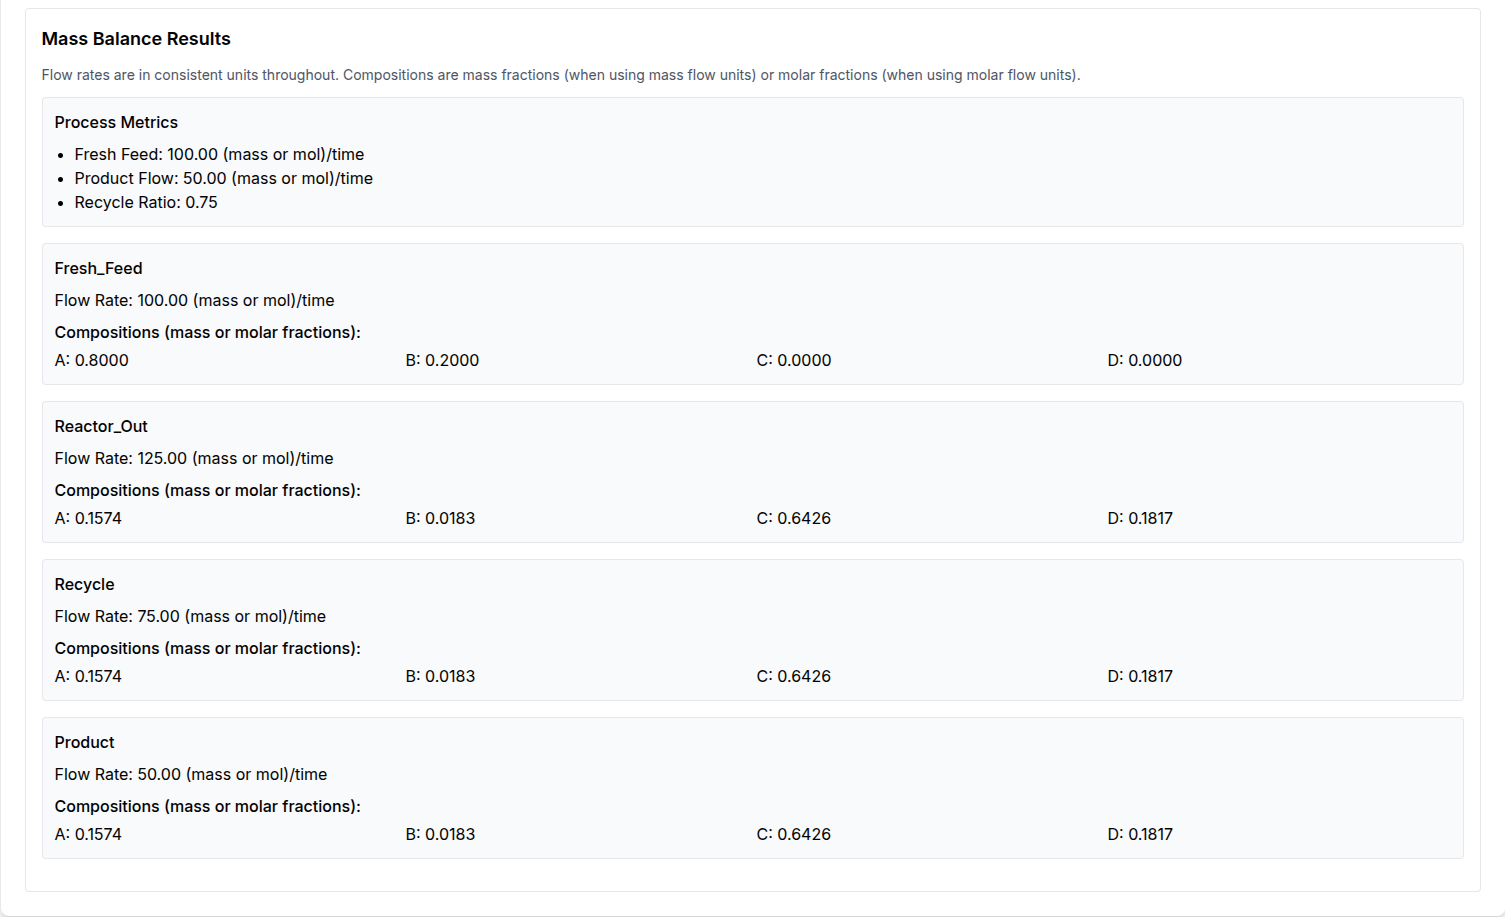
\includegraphics[width=\linewidth]{media/cap4_resultados_balanco_massa_reacao_reciclo.png}
    \fonte{Elaboração própria (2026).}
    \label{fig:mass_balance_results}
\end{figure}

O balanço de massa fundamenta o dimensionamento de equipamentos como misturadores, separadores, reatores e redes de processo, além de embasar análises econômicas (minimizando perdas de matérias-primas) e de segurança (evitando acúmulo indesejado de compostos). Vale notar que temperatura e pressão influenciam o balanço apenas através de propriedades físicas (massa específica, volumes específicos), ou mudanças de fase que afetem as vazões mássicas e molares de cada corrente \cite{felder2005}.

